\chapter{Simulación de la demanda con el MBG}\label{cap:simulacion}

\section{Estructura de covarianza}

El índice de demanda de cada zona sigue \eqref{eq:mbg} con $X_i(2025)=1$ y una estructura de un factor:
\begin{equation}\label{eq:factor}
\sigma_i\,dW_i=\sigma_c\,dW_0+s_i\,dB_i,\qquad
\Sigma=\sigma_c^2\,\mathbf 1\mathbf 1^\top+\diag(s_1^2,\dots,s_Z^2),
\end{equation}
donde $W_0$ es un factor común (ingreso, empleo, tasa de viajes) y $B_i$ son choques locales
independientes. Con $\sigma_c=5\,\%$ y $s_i=3\,\%$ en Bogotá (4\,\% en la región), la volatilidad total
de una zona de Bogotá es \SigmaZona{} anual y la correlación entre zonas de Bogotá es
$0{,}05^2/(0{,}05^2+0{,}03^2)\approx0{,}74$. La deriva $\mu_i$ suma la tendencia demográfica de la zona y
una tendencia común de 0,5\,\% anual en la tasa de viajes motorizados (\cref{tab:zonas}). La deriva
demográfica ponderada de Bogotá es de $-0{,}16\,\%$ anual, consistente con la caída de población que
proyecta el DANE, mientras que los municipios crecen entre 1,2 y 2,0\,\% anual.

\section{Discretización exacta}

Con $L$ el factor de Cholesky de $\Sigma$, la solución \eqref{eq:mbg_sol} da el esquema
\begin{equation}\label{eq:exacta}
\ln X(t_{k+1})=\ln X(t_k)+\big(\mu-\tfrac12\diag\Sigma\big)\Delta t+L\,Z_k\sqrt{\Delta t},\qquad Z_k\sim\mathcal N(0,I),
\end{equation}
que es exacto en distribución para cualquier $\Delta t$: no hay error de discretización como en el
esquema de Euler, solo error de muestreo. Con saltos, se suma $\sum_{j=1}^{N_k}J_j$ a todas las zonas,
con $N_k\sim\text{Poisson}(\lambda\Delta t)$, y la deriva se compensa como en \eqref{eq:merton}. Las
pruebas del paquete verifican que la media y la varianza del logaritmo simuladas coinciden con
$e^{\mu t}$ y $\Sigma_{ii}t$, que la correlación muestral recupera la teórica y que la compensación de
los saltos conserva la media.

\section{Calibración de la volatilidad con TransMilenio}

La serie disponible de demanda troncal de TransMilenio (pasajeros por día hábil) tiene observaciones
irregulares en 2008, 2018, 2019, 2020, 2023, 2024 y 2025 \citep{silla2026}. Con $y=\ln X$, los
incrementos $\Delta y_k\sim\mathcal N(m\,\Delta t_k,\sigma^2\Delta t_k)$ son independientes y los
estimadores de máxima verosimilitud tienen forma cerrada:
\begin{equation}\label{eq:mle}
\hat m=\frac{\sum_k\Delta y_k}{\sum_k\Delta t_k},\qquad
\hat\sigma^2=\frac1n\sum_k\frac{(\Delta y_k-\hat m\,\Delta t_k)^2}{\Delta t_k},\qquad
\hat\mu=\hat m+\tfrac12\hat\sigma^2.
\end{equation}

Con todos los datos, $\hat\sigma=\SigmaTMCompleto$: la estimación está dominada por la caída de
\SaltoTM{} entre 2019 y 2020. Si el choque y el rebote de 2020--2023 se tratan como un salto y se
excluyen de la difusión, $\hat\sigma=\SigmaTMRobusto$ (\cref{fig:mbg_cal}). La deriva de la serie
(\MuTMRobusto{} anual) refleja la expansión de la red entre 2008 y 2018 más que el crecimiento de la
demanda subyacente, por lo que no se usa como deriva del modelo. La lección es doble: la volatilidad de
la difusión es del orden de 5--7\,\% anual, coherente con la calibración por factores, y los choques
sistémicos deben modelarse aparte, como saltos.

\begin{figure}[ht]
\centering
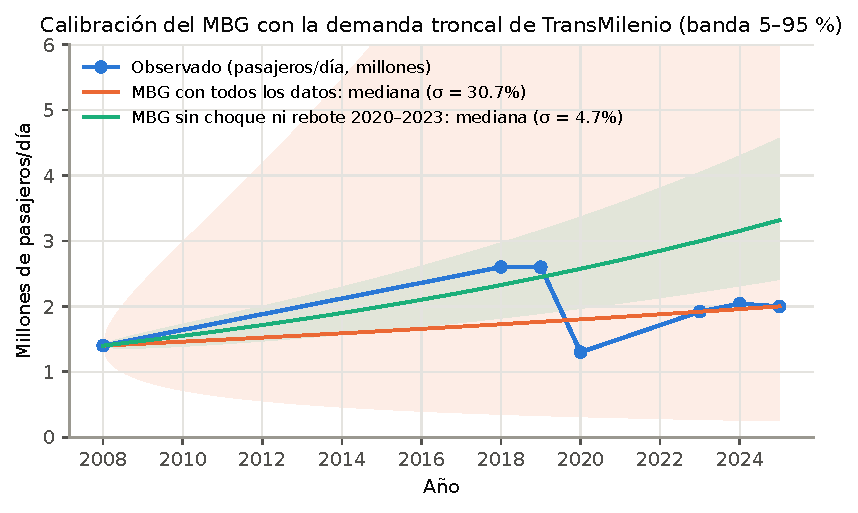
\includegraphics[width=.92\textwidth]{figuras/fig_mbg_calibracion.pdf}
\caption{Calibración del MBG con la demanda troncal de TransMilenio: mediana y banda 5--95\,\% de los
dos ajustes desde 2008.}\label{fig:mbg_cal}
\end{figure}

\section{Escenarios simulados}

El estudio usa $n=\NEscenarios$ escenarios generados con una secuencia de Sobol aleatorizada de
dimensión $25\times12=300$ (semilla \SemillaSimulacion). La \cref{fig:abanico} muestra el índice de
demanda agregado, ponderado por la generación de cada zona, y la \cref{fig:zonas} su distribución por
zona en 2050: la región crece y se dispersa más que Bogotá, y las zonas centrales tienen mediana por
debajo de su nivel actual.

\begin{figure}[ht]
\centering
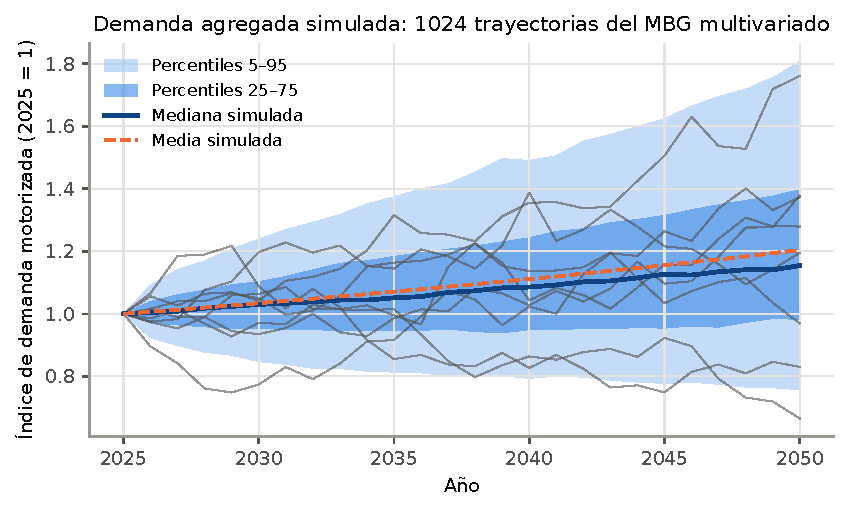
\includegraphics[width=.92\textwidth]{figuras/fig_mbg_abanico.pdf}
\caption{Índice de demanda motorizada agregado: percentiles, mediana, media y ocho trayectorias.}\label{fig:abanico}
\end{figure}

\begin{figure}[ht]
\centering
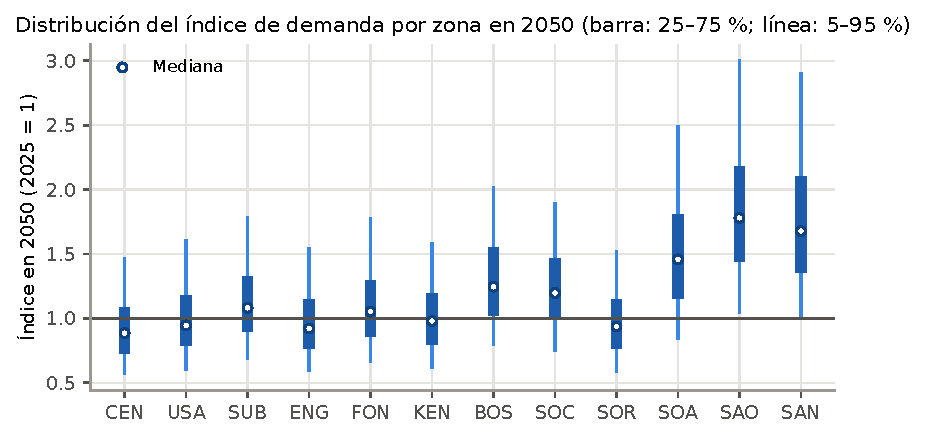
\includegraphics[width=.92\textwidth]{figuras/fig_mbg_zonas.pdf}
\caption{Distribución del índice de demanda por zona en 2050.}\label{fig:zonas}
\end{figure}

\section{Convergencia del estimador}

Para medir el error de muestreo se estimó el costo esperado del diseño base con
$n\in\{32,\dots,\NConvMax\}$ escenarios, veinte réplicas independientes por tamaño y tres métodos, y se
comparó con una referencia de 8.192 escenarios Sobol (\cref{fig:convergencia}). El Monte Carlo
estándar converge con pendiente \PendienteMC{} en escala log-log, cercana al $-1/2$ teórico; las
variables antitéticas tienen pendiente \PendienteAnt{}, y la secuencia de Sobol, \PendienteSobol. Con
$n=\NConvMax$, la raíz del error cuadrático medio pasa de \RMSEMC{} billones con Monte Carlo estándar a
\RMSESobol{} con Sobol, lo que equivale a multiplicar el número de escenarios por cerca de
\GananciaSobol. Frente a diferencias de varios billones entre diseños, ese error es despreciable, y lo
es aún más para las \emph{diferencias} entre diseños gracias a los números aleatorios comunes.

\begin{figure}[ht]
\centering
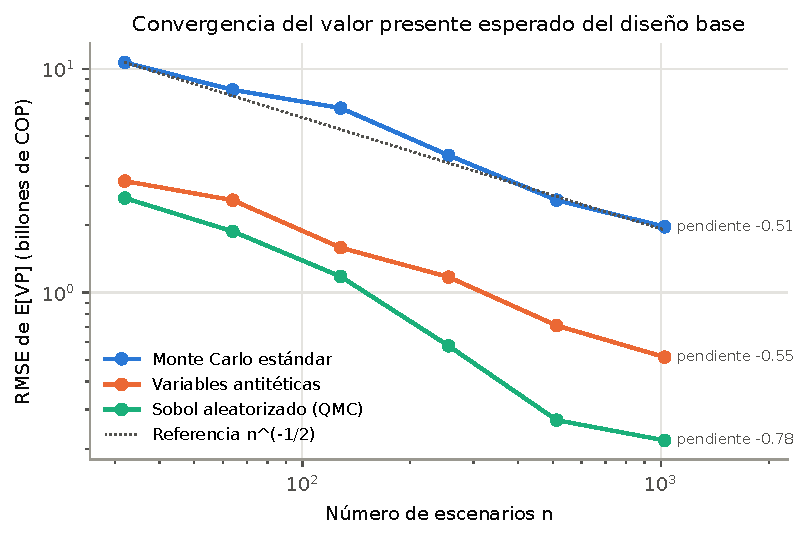
\includegraphics[width=.8\textwidth]{figuras/fig_convergencia.pdf}
\caption{Raíz del error cuadrático medio del costo esperado del diseño base según el método.}\label{fig:convergencia}
\end{figure}
